\chapter{Introduction}

\section{The Hot Big Bang model}

The most accepted model for the origin of the universe is the Big Bang model, which surprisingly to some conveys no "bang", but the sudden existence of all the matter in the universe, in the shortest of times, in the smallest of spaces, about 13.8 billion years ago. After an unthinkably small interval of time, the universe began a short period of rapid expansion known as \textit{cosmic inflation}, in which the universe grew by a factor $10^{27}$ in a mere $10^{-33}$ seconds. This inflation is thought to be due to the inflaton, a quantum scalar field theory. It is theorized that it is the inflaton's vaccuum energy what caused the universe to expand as greatly.

After this inflation phase, the universe cooled enough for what is known as the Quark-Gluon plasma to form. In this state, temperatures were high enough as to consider relativistic the random motion of the particles in it. After some cooling due to cosmic expansion, the combination between quarks to form hadrons was allowed, leading to what is known as the hadronic epoch. However, due to the short mean free path of the photons the universe is still opaque to electromagnetic radiation.

As the universe kept expanding the densities and the temperatures cooled, the existence of atoms was starting to be allowed, the $He^{+}$ and $H$ atoms. This period would finish at the universe age of $380,000$ years, moment known as recombination. Though the name `recombination' implies the fact that the universe used to be `combined' and then ceased to be so, it just comes from the fact that recombination was theorized before the Big Bang theory was thought of.

As soon as recombination ends, the excited electrons which are now orbiting neutral atoms, fall to a lower energy state, thus emmitting photons in great densities. This emmision is known as the Cosmic Microwave Background (CMB) and is the oldest direct measurement we can take of the unvierse.


\begin{figure}[h]
	\centering
	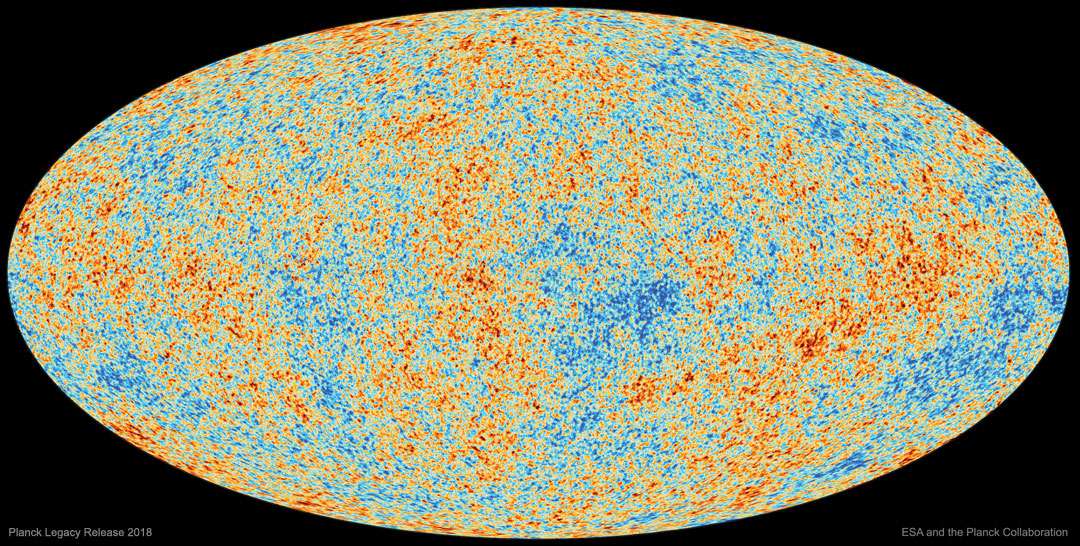
\includegraphics[width=0.8\textwidth]{../figs/cmb.jpeg}
	\caption{The CMB as seen by Space-based Observatory Planck}
	\label{fig:cmb}
\end{figure}
\section{Cosmic Microwave Background}

We see in the figure \ref{fig:cmb} the CMB as observed by the Planck colaboration \cite{Collaboration2018}. The radiaton we observe is the photons that were emmitted about $13.3$ million years ago. Since the CMB appears as a result of the thermal photons emitted by the electrons in the primordial plasma, it offers great insight into what the plasma looked like, and the way it behaved. 

As the name suggests, the CMB radiation consists of wavelengths of radiation of the order of micro meters. In fact, one can measure the associated temperature to this wavelength to be $2.7260$\SI{}{K}\cite{Fixsen2009} with some fluctuations of approximately \SI{0.0013}{K}. However, this is definitely not the temperature of the plasma before recombination. It was in fact, about $2725K$, or $\approx 1000$ times higher. This is due to the process of \textit{cosmological redshift}, which will be explained later on.

A natural question arises: How does this not break the cosmological principle? (i.e. the universe is isotropic and homogenous, meaning it is the same in every direction and at every point in space, respectively)
	
These fluctuations may be explained by the microscopic quantum oscillatios of the different fields that make up matter before and during cosmic inflation. The details of the mechanism that allows a particle to be explained as a field goes way beyond the scope of this paper, so it suffices to just mention the fact that at high enough energies, the concept of particle loses its meaning and it needs to be modeled as a constantly fluctuating field in all of space.

Thus, the CMB becomes crucial in explaining the large scale structure of the universe, since the photons that decoupled from the plasma at recombination wasted more energy leaving denser regions behind losing thermal energy in the process. 

\section{Baryon Acoustic Oscillations}

Before recombination, all matter was coupled into the same fluid which we have called the primordial plasma. The particles in the plasma interacted primarily with one another through gravity and electromagnetism, depending on the type of matter considered. 

As already mentioned, matter was not distributed homogenously so at some point in time before recombination one could find `lumps' of dark and baryonic (standard) matter. Combining the gravitational attraction between dark and baryonic matter with itself and with one another, and the repulsion caused by the Thomson Effect between baryons and photons, the results are acoustic waves propagating through the plasma, with the dark matter lumps being in the center of these waves. 

The waves would propagate throughout the plasma as long as the baryon-photon interaction was strong enough i.e. up until recombination, at which they froze in time leaving high 


El concepto de expansión del universo aparece cuando Erwin Hubble observa que las mediciones de la longitud de onda de radiación de las galaxias alrededor nuestra estaban todas desplazadas hacia el rojo. Es decir, estaban dilatadas. Esto indica que debido a la expansión del universo la longitud de onda de la radiación observada se habrá dilatado. Introducimos así la Ley de Hubble 
\begin{align}
	v = H_0 d
	\label{eq:ley-hubble}
\end{align}
Que nos relaciona la velocidad de expansión de un punto separado una distancia d del observador, a través de la constante de Hubble $H_0 = 100h \frac{km}{s \cdot Mpc}$, siendo $h$ un factor que permite parametrizar nuestro desconocimiento sobre $H_0$. $H_0$ representa realmente el valor actual de $H(t)$, así como cualquier observable cosmológico $A_0$ representa el valor actual de $A(t)$. 

Introducimos así el concepto \textit{redshift} como variable temporal.
\begin{align}
	z = \frac{\lambda_{\text{observado}} - \lambda_{\text{emitido}}}{\lambda_{\text{emitido}}}
	\label{eq:redshift}
\end{align}
La luz necesita tiempo para llegar a su destino, y durante ese tiempo el universo se habrá expandido cierta cantidad. Esa cantidad desplaza la radiación hacia el rojo dándonos una idea de cuánto tiempo ha estado la onda viajando, es decir cuál es la edad del objeto que estamos observando.

La expansión del universo viene parametrizada por un factor de escala $a(t)$, de tal forma que si en cierto momento medimos una distancia $a(t_0)\Delta x$, pasado un cierto tiempo $\Delta t$ la nueva medida de esa misma distancia resultará en $a(t_0+\Delta t) \Delta x$\footnote{Más precisamente, $a(t)$ aparece en la métrica de Friedman-Lemaître-Robertson-Walker (FLRW) 
\begin{align}
	ds^{2} = -dt ^{2} + a^{2}(t) \left( \frac{dr^{2}}{1-kr^2} + r^2d\theta^2 + r^2 \sin ^2 \theta d\phi^2\right) 
\end{align}}

Es decir, que si consiguiésemos averiguar la expresión de $a(t)$, podríamos determinar la historia del universo. Alexander Friedmann desarrolló en 1922 las ecuaciones de Friedmann en las que define formalmente el ya mencionado parámetro de Hubble $H(t)$
\begin{align}
	H^2(t) := \left(\frac{\dot a}{a}\right)^2 &=  \frac{8\pi G \rho}{3} +\frac{  \Lambda c^2}{3} - K \frac{c^2}{a^2}
	\label{eq:1a-friedmann}\\
	3 \frac{\ddot a}{a} &= \Lambda c^2 - 4\pi G \left( \rho + \frac{3p}{c^2} \right) 
	\label{eq:2a-friedmann}
\end{align}
Siendo  $G$ la constante universal de gravitación, $\rho$ la densidad de materia del universo, $\Lambda$ la constante cosmológica, $K$ la curvatura Gaussiana del universo y  $p$ la presión del universo.

Se puede expresar la ecuación \eqref{eq:1a-friedmann} de una forma más legible, definiendo los parámetros 
\begin{align}
\Omega_m = \frac{8\pi G \rho}{3H^2}, \Omega_\Lambda = \frac{\Lambda c^2}{3H^2}, \Omega_K = -K\frac{c^2}{H^2a^2} 
\end{align}
Conocidos como los parámetros de densidad, de vacío y de curvatura. Los dos primeros son los que contienen la información de la densidad de los fotones, neutrinos, bariones, materia oscura y energía oscura.

Reescribimos así la ecuación \eqref{eq:1a-friedmann}
\begin{align}
	1 = \Omega_m + \Omega_\Lambda + \Omega_K
\end{align}
Que es la ecuación que cumplirá cualquier universo que estudiemos, entendiendo por universo o cosmología los diferentes valores que se le den a los parámetros $\Omega$

Con estos conceptos podemos relacionar el \textit{redshift} con el factor $a(t)$ 
\begin{align}
	1+z = 1+  \frac{\lambda_o - \lambda_e}{\lambda_e} = \frac{a(t_o)}{a(t_e)}
	\label{eq:relacion-z-a}
\end{align}
La ecuación \eqref{eq:relacion-z-a} nos permite relacionar el factor de escala actual con el que había en el universo en el momento de emisión de la radiación observada, en función del \textit{redshift}que observemos.

Otra relación importante será también la que nos permite calcular el parámetro de Hubble en función de la cosmología que escojamos 
\begin{align}
	H(z) = H_0 \sqrt{\Omega_m(1+z)^3 + \Omega_K(1+z)^2 + \Omega_\Lambda} 
\end{align}
A través de la constante de Hubble calculamos también la distancia de Hubble 
\begin{align}
	D_H = \frac{c}{H(z)}
	\label{eq:distancia-hubble}
\end{align}
Que actualmente toma un valor de $D_H = 3000h^{-1}\text{Mpc}$. La distancia de Hubble se define como la distancia a partir de la cual la velocidad de expansión del universo relativa al observador es mayor a la velocidad de la luz\footnote{Si sustituimos $v=c$ en \eqref{eq:ley-hubble}, sustituimos $v=c$ y despejamos la D correspondiente queda exactamente la expresión de $D_H$}


Aquí explico los parámetros que afectan a la expansión del universo y por tanto al redshift y por tanto a las medidas que tomamos.


%(condiciones iniciales, expansión del universo, composición del plasma primordial, parámetros cosmológicos LCDM)

\section{Oscilaciones Acústicas de Bariones.}
Las concentraciones de materia implicaban unas intensas interacciones que al equilibrarse con la presión de radiación, daban lugar a la propagación de ondas acústica de manera isótropa por el mencionado plasma, que se propagabn a una velocidad usualmente aproximada según $v = \frac{c}{\sqrt{3} }$. 

\section{El Fondo Cósmico de Microondas.}

\section{La estructura a gran escala del universo.}

\section{La escala BAO como regla estándar.}





%
%\section{Fundamento teórico}
%\subsection{Oscilaciones Bariónicas Acústicas}
%En los primeros cientos de miles de años del universo, éste existía en un estado hiper denso conocido como plasma primordial, formado por (hasta lo que sabemos) materia oscura, bariones y fotones.
%Debido a la alta concentración de materia del universo temprano, había una fortísima atracción gravitatoria, contrarrestada por la presión de radiación debida al Efecto Thomson. 
%
%Las altísimas temperaturas del universo en la época anterior a la recombinación generaban fotones cuya presión de radiación generaba perturbaciones en el plasma que se propaga de forma isotrópica por el espacio.
%Estas ondas acústicas necesitan por supuesto un medio por el que viajar. Al expandirse el unverso disminuyendo así la concentración de materia, llegado cierto punto la distancia entre partículas será demasiado grande como para interactuar, prohibiendo así la expansión de las ondas acústicas y congelándolas en el tiempo.
%Se conoce el radio de estas ondas como la escala acústica o horizonte del sonido $r_{s}\approx 150Mpc$\cite[Eisenstein2004]. 
%
%\subsection{Análisis BAO}
%
%El análisis de oscilaciones acústicas bariónicas (BAO, por sus siglas en inglés) permite, a través de estudios de gran volumen, analizar y medir $r_s$.
%Las oscilaciones BAO no son fáciles de ver a simple vista, pero sabiendo que las galaxias proliferan en esferas de radio $r_s$, se propone la función de correlación a dos puntos $X_i(r)$ que devuelve la distribución de distancias de galaxias. Esto es, dada una galaxia en un punto $\textbf{r}_i$ esta distará del resto de galaxias del universo en posiciones $\{\textbf{r}_j\} $ por una distancia $ \{\|\textbf{r}_i - \textbf{r}_j \|\} $. La densidad $X_i(r)$ recoge la estadística de las distancias a las que se suelen encontrar las galaxias.
%
%Se define $P(k)$ o \textit{galaxy power spectrum} como la transformada de Fourier de $X_i(r)$. Puesto que tenemos un patrón que se repite cada $r_s$, esta función presenta picos en $\frac{2\pi}{r_s}$. 
%
%Al conocer el tamaño \textit{comoving}\footnote{'\textit{Comoving}' hace referencia a lo que mediríamos si el universo no se hubiese expandido} de estas ondas esféricas congeladas en el tiempo, si conseguimos medir su tamaño actual 'físico' (es decir, considerando la expansión del universo) podremos usar esos resultados para tomar medidas más y más precisas de objetos muy distantes. 
%
%La expansión del universo afecta por igual a todas las distancias, incluida la longitud de onda de la luz. Por ello, observaremos una tendencia hacia el rojo de cualquier radiación que midamos, fenómeno conocido como \textit{redshift}. Al conocer el espectro electromagnético de emisión de una galaxia, podemos contrastar la longitud de onda que observamos con la que 'debería ser', es decir, la longitud de onda de emisión. 
%
%Definimos así el ya mencionado redshift $z$
%\begin{align}
%z = \frac{\lambda_{\text{observado}} - \lambda_{\text{emitido}}}{\lambda_{\text{emitido}}}
%\end{align}
%Que se podrá usar como una medida del tiempo que ha estado la onda viajando.
%
%\subsection{Efecto de la curvatura del universo}
%
%A día de hoy, todos los estudios BAO que se han realizado han asumido un universo sin curvatura. Esto es, aunque el universo presenta curvatura de manera local debido a las concentraciones de masa, el universo es plano de manera asintótica. 
%
%
%\subsection{Estudio de las curvas BAO}
%
